% -*-LaTeX-*-

% $Log: filt-intro.tex,v $
% Revision 1.7  2007/12/11 02:10:08  stiber
% All the relatively small modifications for the start of the
% Winter 2008 quarter.
%
% Revision 1.6  2007/03/20 23:52:45  stiber
% Cleaned up and updated LaTeX.
%
% Revision 1.5  2007/03/18 18:56:10  stiber
% Modified file for stand-alone textbook. Checked that it will format
% along with the rest of the book as of this point.
%
% Revision 1.4  2006/03/27 23:36:06  stiber
% Fixed error in formula.
%
% Revision 1.3  2004/05/03 20:13:30  stiber
% Fixed typos and errors in end of chapter problems.
%
% Revision 1.2  2004/03/29 19:53:17  stiber
% Updated for Spring 2004 and new textbook (DSP First).
%
% Revision 1.1  2004/02/19 00:24:08  stiber
% Initial revision
%

\chapter{Filtering and Feedforward Filters}
\label{ch:filt-intro}

% Use the starred versions of section, subsection, etc.
\section{Introduction}

In this chapter, we will introduce you to the most basic type of
algorithm for processing digital signals: feedforward filters. We
start with the concept of \emph{filtering} and the operation of basic
feedforward filters. By the end, you should understand some important
terms related to filters, for example, \emph{frequency response},
\emph{phase response}, \emph{transfer function} and \emph{zeros} of a
\emph{transfer function}. You should be able to implement simple
digital filters on a computer and use them to solve some simple signal
processing problems.

The concept of filtering should not be new to you. For example, if you
were interested in filtering and opened this book, you would see that
this chapter deals with filtering and so you would pay attention to
this chapter and ignore the others.  Your mind performed a
\emph{bandpass} filter with the pass \index{filter!bandpass} band
being chapter \ref{ch:filt-intro}.  Some other kinds of filters are
\emph{low pass}, \emph{high pass}, and \emph{band stop}.  Using the
same example, a low pass filter \index{filter!low pass} allows you to
attend to all the chapters in the book, from the beginning to the end
of the pass band, say chapter~\ref{ch:filt-intro}; the high pass on
\index{filter!high pass} the other hand will pass only the chapters
beyond a certain one, say beyond chapter 4; the band stop is the one
\index{filter!band stop} that allows you to pay attention to all the
chapters \emph{except} the stop band, say chapter \ref{ch:filt-intro}.

In the signal processing domain, filters exclude and/or include signal
\emph{frequencies}. For example, consider a signal $x(t)$ (where $t$
is time) with four sinusoidal components. It has frequencies at
$f_1=50$, $f_2=100$, $f_3=250$, and $f_4=350$:

\begin{equation}
x=\sin(2\pi t f_1)+\sin(2\pi t f_2)+\sin(2\pi t f_3)+\sin(2\pi t f_4)
\label{eq:sine4}
\end{equation} 

\problemset{
\subsubsection{Self-Test Exercise}

See~\ref{sc:ch3ex} \#\ref{it:ch3ex0} for the answer.

\begin{enumerate}
\item Is the signal of equation~\ref{eq:sine4} periodic? If so, what
  is its period?
\end{enumerate}}

\begin{figure}
\centerline{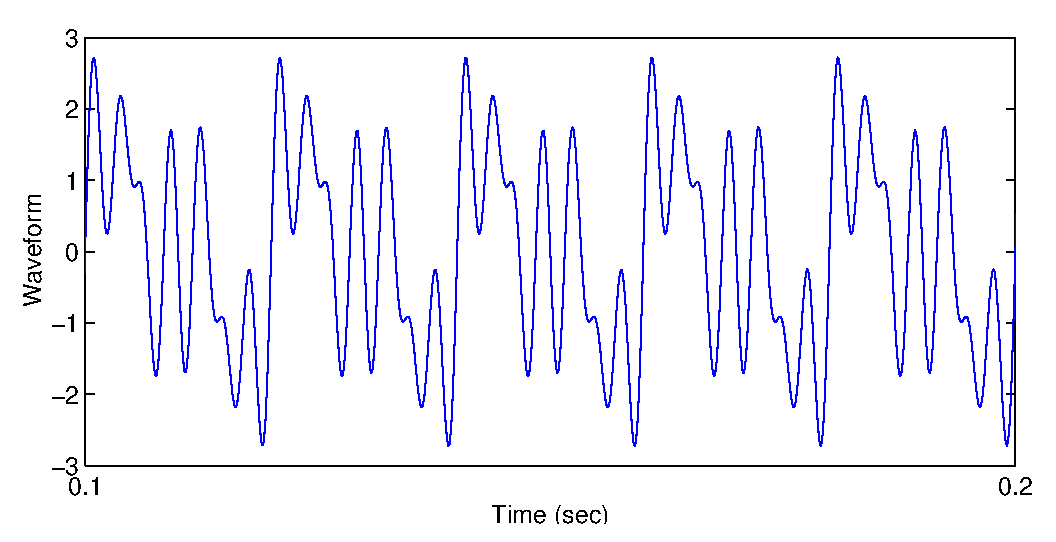
\includegraphics[width=5in]{ch-fir/sine4}}
\caption[Four frequency components]{A sinusoidal signal with four
frequency components: $f_1=50$, $f_2=100$, $f_3=250$,
$f_4=350$Hz.\label{fig:sine4}}
\end{figure}

Figure~\ref{fig:sine4} shows a plot of about 0.1 second of this
signal. Its four frequencies are shown as green peaks in
figure~\ref{fig:sine4-sp}.  Let's say that we would like to have a
filter to keep the $f_3=250$Hz sinusoid and get rid of the $f_1$,
$f_2$, and $f_4$ sinusoids. This filter can be visualized as in
figure~\ref{fig:sine4-band}. Here, the horizontal axis is frequency
and the vertical axis is magnitude of the filter's response. The
filter is designed to have a frequency passband between 200 and 300
Hz, which means that only the signal's frequency components within
this band are allowed to pass. Figure~\ref{fig:sine4-f2} shows this
filter's output --- in other words, the filtered signal --- plotted
along time. Another way to look at the filtered signal is its
frequency components, which are shown in figure~\ref{fig:sine4-sp}
(magenta). This latter graph clearly shows that, after filtering, the
signal is very close to a 250 Hz sinusoid, exactly as expected.  You
can hear these two signals as sounds:
\url{http://courses.washington.edu/css457/ebook/sine4.au} is the sum
of four sinusoids and
\url{http://courses.washington.edu/css457/ebook/filtered_sine4.au} is
the filtered version.  \index{audio files!sinusoids} \index{audio
  files!filtering}

\begin{figure}
\centerline{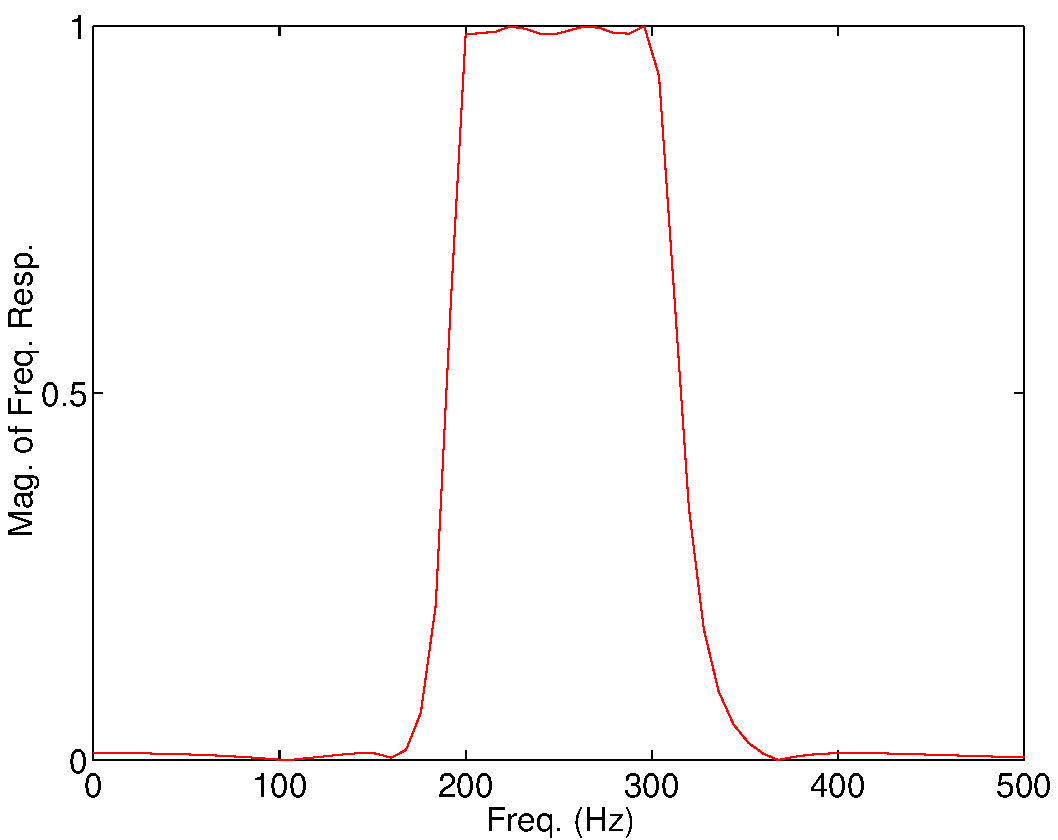
\includegraphics[height=3in]{ch-fir/sine4_band200-300}}
\caption[Filter frequency response]{Filter's frequency response. The
pass band is [200 300] Hz.\label{fig:sine4-band}}
\end{figure}

\begin{figure}
\centerline{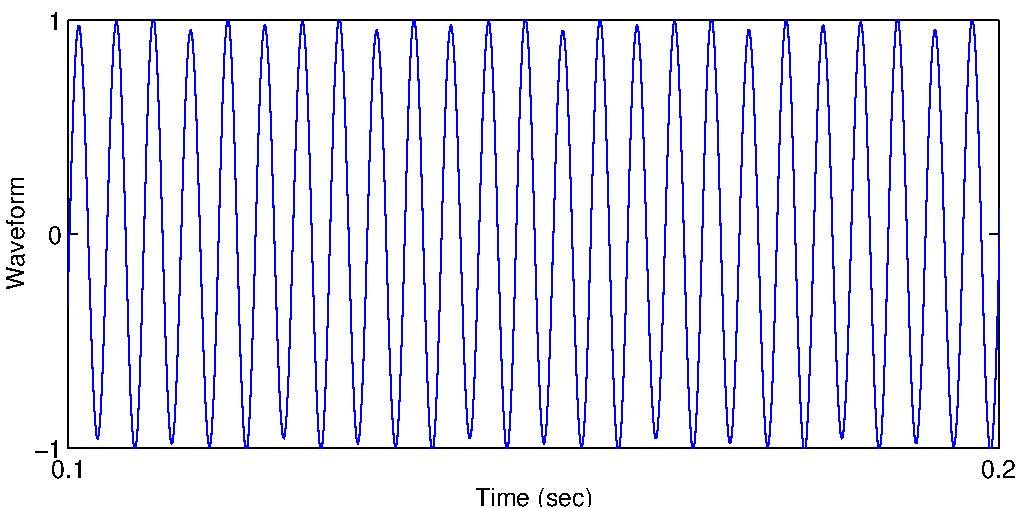
\includegraphics[width=5in]{ch-fir/sine4_filted}}
\caption[A filtered signal]{The signal~(\protect\ref{eq:sine4}) after filtering out
frequencies 50, 100 and 350Hz.\label{fig:sine4-f2}}
\end{figure}

\begin{figure}
\centerline{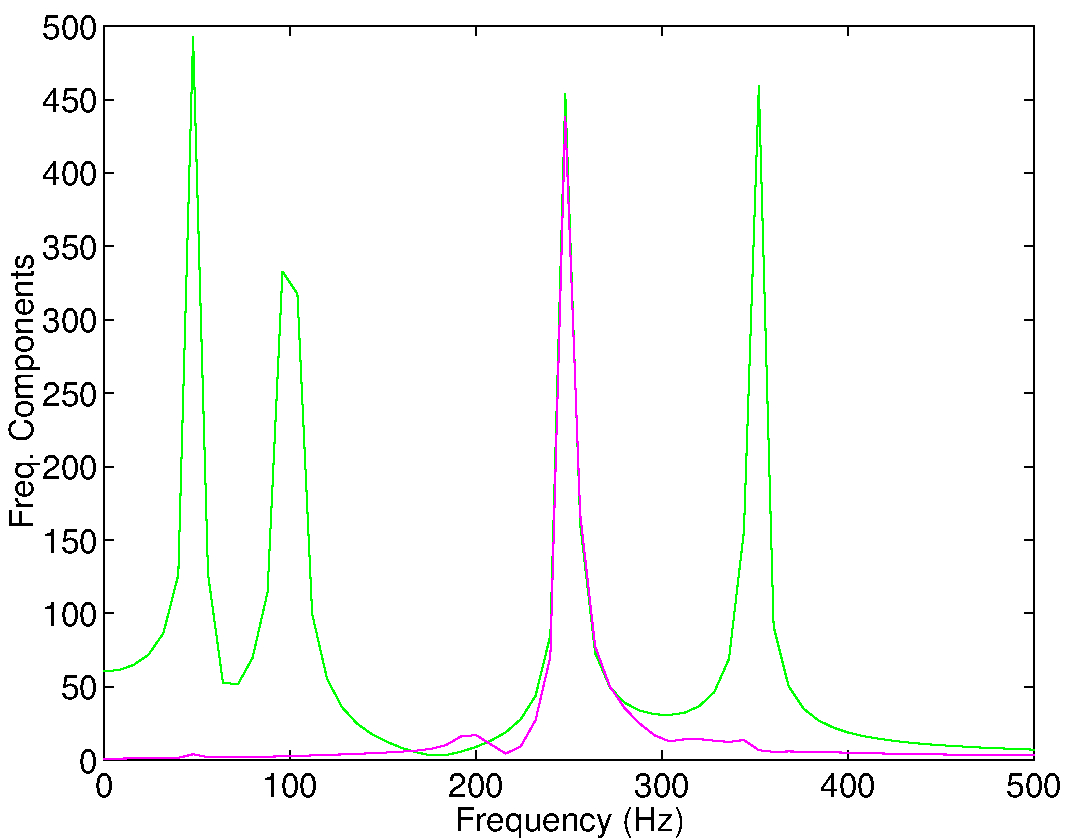
\includegraphics[height=3.5in]{ch-fir/sine4_sp}}
\caption[Unfiltered vs. filtered signal]{Spectrum of four-sinusoid
signal (green) and its filtered version
(magenta).\label{fig:sine4-sp}}
\end{figure}

At this point, you should have an idea of what filters do. Next, I
will explain \emph{how} filters work.

\section{Feedforward Filters}

\subsection{Delaying a phasor}

In chapter~\ref{ch:physical-signals}, we learned the term
\emph{phasor}, a complex sinusoid expressed as $e^{j\omega t}$.  We
also saw that this representation makes the math simpler for adding
sinusoids, at least.  A phasor's magnitude is one, its frequency is
$\omega$, and it angle is $\omega t$, where $t$ is time. It moves
around the unit circle counter-clockwise along time.  If we delay it
by $\tau$ sec, then the delayed time is $t-\tau$, and we can write
this as:

\begin{equation}
e^{j\omega (t-\tau)} = e^{-j\omega \tau} e^{j\omega t}
\end{equation}

This is the product of two phasors at the same frequency.
This doesn't do anything except rotate the phasor by $-\omega \tau$
(i.e., it doesn't change its magnitude).

\subsection{A simple feedforward filter}

\begin{figure}
\centerline{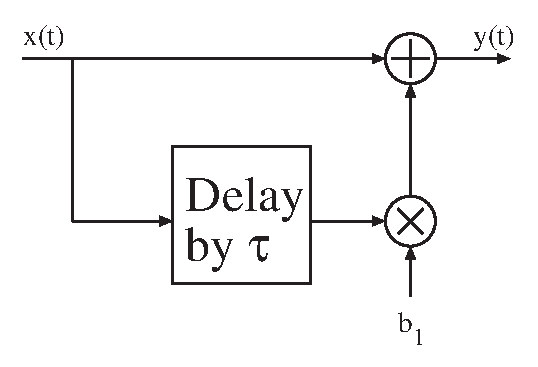
\includegraphics[width=0.5\textwidth]{ch-fir/ff-bdiag}}
\caption{A basic feedforward filter block diagram.
  \label{fig:ff-bdiag}}
\end{figure}

Filters combine delayed versions of signals. We have already seen that
signals are made up of phasors. A simple feedforward filter's
\emph{block diagram} is shown in figure~\ref{fig:ff-bdiag}.
\index{block diagram}
\index{diagram!block}
A block diagram is a type of data flow diagram: it shows flow of
\index{data flow diagram}
\index{diagram!data flow}
signal \emph{data} within the filter (in contrast to a \emph{flow chart}, which
\index{flow chart}
\index{diagram!flow chart}
shows flow of \emph{control} within a program. In
figure~\ref{fig:ff-bdiag}, the input signal data $x(t)$ branches, with
one copy sent to an adder (``+'') and another sent to a delay
block. The output of the delay block is sent to a multiplier, which
multiplies it by the constant $b_1$ (sometimes, multiplication by a
constant is just indicated by writing the constant next to a
link). 
Its output, $y(t)$, is the summation of its input and a
scaled (or \emph{weighted}) version of its input delayed by
$\tau$. Given an input signal $x(t)$, its delayed version $x(t-\tau)$,
and coefficient $b_1$, the output $y(t)$ can be written by inspection
of the block diagram as:
\begin{equation}
y(t) = x(t) + b_1 x(t-\tau) \label{eq:ff-filt-gen}
\end{equation}
When the input is a phasor, $x(t) = e^{j\omega t}$,
equation~(\ref{eq:ff-filt-gen}) becomes:
\begin{equation}
y(t)=e^{j\omega t} + b_1 e^{j\omega (t-\tau)}
\label{eq:ff-filt-ph}
\end{equation}

Notice that the input and the output have the same frequency,
$\omega$. We can factor out the $e^{j\omega t}$ in
equation~(\ref{eq:ff-filt-ph}) to obtain:
\begin{align}
y(t) &= [1 + b_1 e^{-j\omega \tau}] e^{j\omega t}\\
&= \mathcal{H}(\omega) e^{j\omega t} \label{eq:fresp-mult} \\
&= \mathcal{H}(\omega) x(t)
\end{align}
where 
\begin{equation}
\mathcal{H}(\omega) = \frac{y(t)}{x(t)} = 1+b_1 e^{-j\omega \tau}
\end{equation}
\index{filter!frequency response|emph}%
is called the filter's \emph{frequency response}: how its output
varies as a function of the input frequency (i.e., the ratio of output
to input). Remember that $\tau$
\index{frequency response}
is a constant delay; what can vary here (besides $t$, which is the
same for both $x(t)$ and $y(t)$) is the frequency of the input,
$\omega$. So, $\mathcal{H}(\omega)$ is a complex function of frequency.
Frequency response is generally written in a polar form with its
magnitude response $|\mathcal{H}(\omega)|$ and phase response
$\theta(\omega)$:
\index{magnitude response}
\index{phase response}
\begin{equation}
\mathcal{H}(\omega)= |\mathcal{H}(\omega)|e^{-j\theta(\omega)}
\label{eq:fresp-polar}
\end{equation}

According to equations~(\ref{eq:fresp-mult})
and~(\ref{eq:fresp-polar}), for a given input sinusoid at frequency 
$\omega$, the filter scales the amplitude by its
magnitude response $|\mathcal{H}(\omega)|$ and shifts its phase by the
phase response $\theta(\omega)$. These two functions  completely define the
filter's behavior. For this particular example, considering only the
magnitude,
\begin{align}
|\mathcal{H}(\omega)| &= |1+b_1 e^{-j\omega \tau}| \label{eq:ff-mha}\\
           &= |1+b_1^2 + 2b_1 \cos(\omega\tau)|^\frac{1}{2}
\label{eq:ff-mh}
\end{align}
(leaving the derivation to an upcoming self-test exercise).

Since $|\cos(\omega\tau)|\leq 1$, the maximum value
$|\mathcal{H}(\omega)|$ can reach is $(1+b_1)$, which occurs when the
angle $\omega\tau=n\pi, n=0,2,4,...$ (zero or even multiples of
$\pi$). Why is this (answer in~\ref{sc:ch3ex} \#\ref{it:ch3ex1})?
Similarly, the minimum of $|\mathcal{H}(\omega)|$ is $1-b_1$, which
happens when $\omega\tau=n\pi, n=1,3,5...$ (odd multiples of $\pi$).
For example, let's say $\tau=167 \mu$s.  Remembering that $\omega$
(radians/second) is converted to Hz by $\omega=2\pi f$, this delay
corresponds to a filter with passbands centered at $2\pi f \tau =
n\pi$, or $f = n/(2\tau)$ for even $n$, producing maxima at 0,
$1/\tau$ (6 kHz), and $2/\tau$ (12 kHz) and notches at $f = n/(2\tau)$
for odd $n$, or $1/(2\tau)$ (3 kHz), $3/(2\tau)$ (9 kHz), and
$5/(2\tau)$ (15 kHz).

You can easily see how the input signal's frequency components
(remember that all periodic functions can be expressed as sums of
complex sinusoids) will be altered by the filter: when they are within
the filter's passbands, they will be passed through; they will be
reduced in magnitude or filtered out when their frequency matches the
low magnitude response. Figure~\ref{fig:sine4-band} is another example
of a bandpass filter with passband [200 300] Hz. The input signal's
frequencies out of this range are filtered out. This is shown in
figure~\ref{fig:sine4-sp}: in the output signal, only the frequency
component at $f=250$ Hz is left.

\problemset{
\subsubsection{Self-Test Exercise}

See~\ref{sc:ch3ex} \#\ref{it:ch3ex2} for the answer.

\begin{enumerate}
\item Use Euler's formula and the definition of the magnitude of a
complex vector to derive~(\ref{eq:ff-mh}) from~(\ref{eq:ff-mha}).
\end{enumerate}}

\subsection{Digital Filters}

Electrical engineers have spent a lot of time developing different
kinds of filter transfer functions for different classes of filters.
You may run across names like Butterworth or Chebyshev. The motivation
behind this has been to produce filters with good properties (flatness
of the passband, steepness of the rolloff from the passband, minimal
phase distortion) that is still implementable in analog hardware
(operational amplifiers, resistors, and capacitors). However, once we
digitize a signal, we can filter it in a computer because filtering is
a mathematical operation and that's what computers do. By directly
implementing a filter's frequency response, we can implement digital
filters that may be difficult or impossible to implement in analog
hardware.

To be implemented on a computer, an analog filter must be discretized
in its variables, to yield a \emph{digital filter}. There are two
\index{filter!digital}
important points here related to digital filters compared to analog
filters:

\begin{enumerate}
\item Time is expressed as an integer times a \emph{sampling period}, $T_s$.
\item Only frequencies below the \emph{Nyquist frequency} can be
represented.
\end{enumerate}
\index{sampling period}

For the first point, recall that digitized time $t$ or $\tau$ is in form of:
\begin{align}
t=n T_s &&\text{(digital time)}
\end{align}
or, 
\begin{align}
\tau=m T_s &&\text{(digital delay)}\label{eq:digital-tau}
\end{align}
where $n$ and $m$ are integers, and $T_s$ is the time interval between
samples or the sampling period, whose units are sec/sample. Note in
equation~(\ref{eq:digital-tau}) that we can only delay a digital
signal by an integer number of sampling intervals. When the
\emph{sampling rate} is $f_s$ (samples/second), $T_s=1/f_s$. 
\index{sampling rate}
So the phasor becomes $e^{j\omega t} = e^{j\omega n T_s}$, with its
exponent having units of radians/sec $\times$ samples $\times$
sec/samples = radians.

\begin{window}[0,r,%
\sidebar{\textbf{Units:}\\
\begin{tabular}{ll}
$T_s$ & seconds/sample \\
$f_s$ & samples/second \\
\hline
$t$ & seconds \\
$f$ & cycles/second (Hz) \\
$\omega$ & radians/second \\
$f_\mathit{Nyquist} = 1/2f_s$ & cycles/second \\
\hline
$n$ & samples \\
$\hat{\omega}$ & radians/sample \\
$\hat{\omega}_\mathit{Nyquist} = \pi$ & radians/sample \\
$\hat{f}$ & cycles/sample \\
$\hat{f}_\mathit{Nyquist} = 1/2$ & cycles/sample 
\end{tabular}},{}]
It's rather cumbersome to have to carry around $T_s$ or $f_s$ in all
our equations.  Additionally, if we keep these variables we will
always need to note and remember the signal in question's Nyquist
frequency. To simplify our notation, let's again use our notion of digital frequency,
$\hat{\omega}$. Recall that $\hat{\omega}=\omega T_s$ and is a \emph{normalized frequency} on the interval $-\pi$ to $\pi$ (with units of
radians/sample). Using this notation we only need to use the sample index $n$, rather than the analog
time $t$. Similarly, our normalized frequency will be
$\hat{f}=fT_s=f/f_s$, with units of cycles/sample.  Our phasor then
becomes $e^{j\omega nT_s}=e^{j\hat{\omega}n}$, and has the same form as the analog
version, except that we are now using the sample index instead of
continuous time.
\end{window}

\index{Nyquist limit}
For the second point, recall that the Nyquist frequency is:
\begin{equation}
f_\mathit{Nyquist}=\frac{f_s}{2}
\end{equation}
Only frequencies below $f_\mathit{Nyquist}$ will be accurately
represented after sampling, beyond it they are aliased to frequencies
below $f_\mathit{Nyquist}$. It is important to restrict the frequency
range to $f_\mathit{Nyquist}$ so you can get correct results.

Again, for convenience, the digital frequency can be normalized by
$f_s$,
\begin{equation}
\hat{f} = \frac{f}{f_s}
\end{equation}
and 
\begin{equation}
\hat{f}_\mathit{Nyquist}=\frac{f_\mathit{Nyquist}}{f_s}=\frac{f_s/2}{f_s}=\frac{1}{2}
\end{equation}
Since the analog $f \leq f_s/2$, $\hat{f}$ is a fraction that ranges
between zero and 1/2 --- a fraction of the digital sampling rate. In
other words, for a sinusoid, we can only have up to 1/2 of a cycle per
sample. We can multiply it by $f_s$ to convert it back to the analog
units of Hz, if necessary.

If $\hat{f}_\mathit{Nyquist}$ is 1/2, the normalized
$\hat{\omega}_\mathit{Nyquist}$ is
\begin{equation}
\hat{\omega}_\mathit{Nyquist} = 2\pi \hat{f}_\mathit{Nyquist}= 2\pi \times 1/2 = \pi 
\end{equation}
%
This explains why $\hat{\omega}$ is always between $-\pi$ and $\pi$ and why $\hat{f}$ is always between $-1/2$ and $1/2$ (its Nyquist!). Going back to our simple feedforward filter, the discrete
representation of equation~(\ref{eq:ff-mh}) with a one time step delay
($\tau = T_s$) is:
\begin{equation}
|\mathcal{H}(\hat{\omega})|=|1+b_1^2 + 2b_1
\cos(\hat{\omega})|^\frac{1}{2}
\end{equation}
When $\hat{\omega}$ is zero, $|\mathcal{H}(0)|=(1+b_1)$. When $\hat{\omega}=\hat{\omega}_\mathit{Nyquist}=\pi$,
$|\mathcal{H}(\hat{\omega}_\mathit{Nyquist})|=(1-b_1)$. The response begins with a large magnitude and reaches a minimum at $\hat{f}=1/2$ (the maximum digital frequency).
The filter has a broad band from 0 until the minimum, so it can pass all
the frequencies from 0 to below 1/2 --- this filter is a lowpass
filter!

\problemset{
\subsubsection{Self-Test Exercises}

See~\ref{sc:ch3ex} \#\ref{it:ch3ex2.2}--\ref{it:ch3ex2.3} for answers.

\begin{enumerate}
\item Suppose that we sample a signal at 1000Hz. For each of the
  following analog frequencies $f$, determine $\omega$,
  $\hat{f}$, and $\hat{\omega}$. Indicate if that frequency will be
  aliased.
  \begin{enumerate}
  \item $f=100$Hz.
  \item $f=200$Hz.
  \item $f=500$Hz.
  \item $f=1000$Hz.
  \end{enumerate}
\item Suppose that we sample a signal at 44.1kHz (the sampling rate
  used in audio CDs). For each of the following analog frequencies
  $f$, determine $\omega$, $\hat{f}$, and $\hat{\omega}$. Indicate if
  that frequency will be aliased.
  \begin{enumerate}
  \item $f=100$Hz.
  \item $f=1000$Hz.
  \item $f=10000$Hz.
  \item $f=20000$Hz.
  \item $f=25000$Hz.
  \end{enumerate}
\end{enumerate}}


\subsection{Delay as an Operator} 

We're still on our quest to make the mathematics of filter design and
analysis as simple as possible.  Generally, a feedforward filter can
have many delays, not just one, and the input $x[n]$ to output
$y[n]$ relation can be written as:
\begin{align}
y[n] &= b_0x[n] + b_1x[n-1] + \cdots + b_Mx[n-M] \notag\\
     &= \sum_{k=0}^M b_k x[n-k]
\end{align}
where $M$ is the number of delays. We shall refer to this as the
filter's \emph{defining equation}.
\index{defining equation}
\index{equation!defining}
Each term in the summation corresponds to a parallel pathway in the
block diagram with a particular delay and constant multiplier.

When $x[n]$ is the phasor $e^{jn\hat{\omega}}$ this becomes
\begin{align}
y[n] &= \sum_{k=0}^M b_k e^{jn\hat{\omega} - jk\hat{\omega}}\\
     &= e^{jn\hat{\omega}}\sum_{k=0}^M b_k e^{-jk\hat{\omega}}\\
     &= \underbrace{x[n]\vphantom{\sum_{k=0}^M b_k
          e^{-jk\hat{\omega}}}}_{\text{original signal}}
        \quad\underbrace{\sum_{k=0}^M b_k
          e^{-jk\hat{\omega}}}_{\text{delaying terms}}
\label{eq:ff-manyk}
\end{align}

Now that you're comfortable with the concept of multiplication by the
phasor $e^{-jk\hat{\omega}}$ being a delay, let's get rid of
it. Seriously, though, it's a lot of writing; this phasor is acting as
an \emph{operator} which, when applied to another phasor, delays
it. It is customary to use another symbol for convenience's sake. In this case, we
define an \emph{operator} $z$ as follows:
\begin{equation}
z = e^{j\hat{\omega}}
\end{equation}
\index{z@$z$!delay operator}

\index{operator!mathematical|(}
This is a symbol that represents the application of an action on an
object (an operation, so $z$ is an operator). So a $k$ time delay
$e^{-jk\hat{\omega}}$ can be written as
\begin{equation}
z^{-k} = e^{-jk\hat{\omega}}
\end{equation}

Here $z^{-k}$ is a $k$ time \emph{delay operator}, where $k=0, 1, 2,
\ldots $ denotes the $0, 1, 2, \ldots k, \ldots$ time step
delay. Operators are a general concept in mathematics, which can be
used in many other circumstances to simplify notation.
\index{operator!delay}

\paragraph*{Example 1:}

Consider a ``square'' operator $S$, which squares the thing on which
it operates.  When it operates on a variable $x$, we get:
\begin{equation*}
Sx = x^2
\end{equation*}

\paragraph*{Example 2:}

The transpose operator $\mathsf{T}$ is commonly used in linear
algebra.  It \emph{transposes} the matrix to which it is applied,
exchanging its rows and columns. For example, when applied to the
matrix $\mathbf{A}$,
\begin{equation*}
A=\left[
\begin{array}{ccc}
1 & 2 & 3 \\
4 & 5 & 6 \\
7 & 8 & 9 \\
\end{array}
\right]
\end{equation*}
the result is
\begin{equation*}
\mathsf{T}\mathbf{A} = \mathbf{A}^\mathsf{T} = \left[
\begin{array}{ccc}
1 & 4 & 7 \\
2 & 5 & 8 \\
3 & 6 & 9 \\
\end{array}
\right]
\end{equation*}
\index{operator!mathematical|)}

An operator can be thought of as purely notation (though this can be a
subtle point): it stands for a mathematical operation. We could use a
functional notation, for example $\mathrm{delay}(x[n])$ just as
well. However, if the mathematical operation has certain properties,
then the operator notation is much more useful, as its syntax gives us
``direct access'' to these properties because of our familiarity with
them from other mathematical operations. In the case of delay, the
$z^{-k}$ operator notation ``works'' because of the properties of
multiplication and division on exponents (exponents
add during multiplication; exponents are negated when dividing). We
are not ``really'' multiplying or dividing, in the true sense of
mathematical multiplication and division operations. 
Instead, we are applying the delay operator or its inverse because it ``looks like''
multiplication or division.

\begin{sloppypar}
  Now we're ready to analyze how a digital filter responds to an
  input.  Let the vector $X=\{x[0], x[1], \ldots, x[n], \ldots\}$ be
  the entire digital input signal: the ordered set of all samples.  We
  use the same notation to produce the vector $Y$ for the ordered set
  of output samples. Instead of using just one sample ($x[n]$ and
  $y[n]$) as in equation~(\ref{eq:ff-manyk}), let's substitute $X$ and
  $Y$ and the delay operator $z^{-k}$ to obtain an equation that
  describes the action of a filter on an entire digital signal (in
  other words, how to compute \emph{all} of the elements of $Y$
  ``simultaneously'' using a single parallel operation):
\begin{align}
Y &=\sum_{k=0}^M b_k z^{-k} X\\
  &= [b_0 + b_1z^{-1} + \cdots + b_k z^{-k} + \cdots]X
\end{align}
\end{sloppypar}

The benefit of using the delay operator is that it makes the task of
factoring out the entire signal $X$ simple. If we call the expression
in the square brackets $H(z)$,
\begin{align}
H(z) &= \sum_{k=0}^M b_k z^{-k}\\
     &= b_0 + b_1z^{-1} + \cdots + b_k z^{-k} + \cdots
\end{align}
we get
\begin{equation}
Y = H(z)X
\end{equation}

$H(z)$ is also an operator, which transfers the input signal
$X$ to the output signal $Y$, so it is called the filter's
\emph{transfer function}. 
\index{filter!transfer function|emph}%
\index{operator!transfer function}%
The relation between the analog frequency
response and digital transfer function is
\begin{equation}
\mathcal{H}(\hat{\omega}) = H(z)|_{z=e^{j\hat{\omega}}}
\end{equation}
So, we evaluate the transfer function $H(z)$ at the frequency
$\hat{\omega}$ by substituting $z=e^{j\hat\omega}$ to get the
frequency response.
For $M=1$ (a filter with a single delay), this yields
\begin{equation}
Y = H(z)X = [b_0 + b_1z^{-1}]X \label{eq:one-delay}
\end{equation}
Equation~(\ref{eq:one-delay}) says that the output equals the weighted
sum of the input signal and the input signal delayed by one time step
(one sampling interval).

\begin{figure}
\centerline{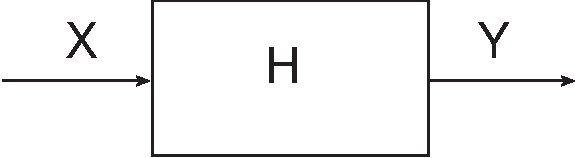
\includegraphics[width=0.5\textwidth]{ch-fir/ff-blackbox}}
\caption{Treat transfer function as a black box.
\label{fig:ff-blacbox}}
\end{figure}

We can treat the transfer function as a black box that does everything
that the filter needs to do. We only need to pay attention to the
input and output, as in figure~\ref{fig:ff-blacbox}.  This give us a
way to combine different filters, simply by composing block
diagrams. Consider two simple filters $H_1(z)$ and $H_2(z)$ connected
in series. $H_1(z)$ has input $X$ and output $W$, and $H_2(z)$ takes
$H_1(z)$'s output as its input and outputs $Y$. Starting from the
output of this system, this can be written
\begin{equation}
Y = H_2(z)W = H_2(z)[H_1(z)X]
  = \underbrace{[H_2(z)H_1(z)]}_{\text{combined transfer function}} X
\end{equation}

This suggests that the combined transfer function is
$H_2(z)H_1(z)$. In fact, we can interchange the order
\begin{equation}
H_2(z)H_1(z) = H_1(z)H_2(z)
\end{equation}
Because the transfer function is a polynomial, this gives us a way to
represent digital filtering as just multiplication by a polynomial
(and the product of two polynomials is just another polynomial).

\problemset{
\subsubsection{Self-Test Exercises}
\label{sc:ste-oper}

See~\ref{sc:ch3ex} \#\ref{it:ch3ex3}--\ref{it:ch3ex5} for answers.

\begin{enumerate}
\item Write equation~(\ref{eq:ff-manyk}) for $k=0, 1, 2, 3$, then
  write the transfer function for each.
\item Given the signal $x(t) = \sin t$ and the derivative operator
  $D=\derivin{}{t}$, what is $Dx(t)$?
\item When
  \begin{align*}
    H_1(z) &= b_0 + b_1z^{-1}\\
    H_2(z) &= b'_0 + b'_1z^{-1}
  \end{align*}
  and $b_0$, $b_1$, $b'_0$, and $b'_1$ are constants, show that
  $H_2(z)H_1(z) =
  H_1(z)H_2(z)$.
\end{enumerate}}

\subsection{The z-plane}

\index{z@$z$!complex plane}
We just used $z$ as a delay operator without much comment as to why we
picked it. In mathematics, the same symbol is used for the complex plane (also called the z-plane).  The
operator $z=e^{j\hat{\omega}}$ is a complex variable in the
z-plane. For any value of $\hat{\omega}$, it lies on a circle of radius one,
at an angle of $\hat{\omega}$ relative to the positive real axis --- it is
the polar representation of a complex number with a magnitude of one. As $\hat{\omega}$ varies from
zero to $2\pi$ (or $-\pi$ to $+\pi$, if you prefer not to consider
$\hat{\omega} > \hat{\omega}_\mathit{Nyquist}$), its path is the unit circle in
the z-plane. Since the Nyquist frequency
$\hat{\omega}_\mathit{Nyquist}=\pi$, we are only interested in the top of half
of the circle running from $\hat{\omega}=0$ to $\hat{\omega}=\pi$.

Using the complex plane makes filters easier to analyze (just like phasors!). To understand why, we will need to develop the relationship between the frequency response of a filter and the complex plane. Let's examine the defining equation of a simple digital filter with
one time delay:
\begin{equation}
y[n] = x[n]-b_1x[n-1]
\end{equation}
Just for convenience, we have used subtraction instead of summation
(or, equivalently you can think of using a negative weight on the
delayed signal). Using the delay operator $z$ and the transfer
function $H(z)$, this becomes:
\begin{equation}
Y = [1-b_1z^{-1}]X = H(z)X
\end{equation}
Obviously,
\begin{equation}
H(z) = 1-b_1z^{-1} = (1-b_1z^{-1}) \frac{z}{z} = \frac{z-b_1}{z}
\end{equation}

For our purposes, we shall restrict ourselves to considering $z$ to be
on the unit circle ($z=e^{j\hat{\omega}}$). The magnitude of $H(z)$ is
the same as the magnitude of $\mathcal{H}(\hat{\omega})$, so the
magnitude of the frequency response is
\begin{equation}
|\mathcal{H}(\hat{\omega})| = |H(z)|_{z=e^{j\hat{\omega}}}
       = \frac{|z-b_1|_{z=e^{j\hat{\omega}}}}{|z|_{z=e^{j\hat{\omega}}}}
       = |z-b_1|_{z=e^{j\hat{\omega}}}
\label{eq:ff-simplez}
\end{equation}
You can see that
although $z=0$ makes the denominator of $H(z)$ zero, we're not
considering that case --- we've already said that we're on the unit
circle: that $|z|=1$.  The value that makes the denominator of
$H(z)$ zero is called a \emph{pole}, which we will talk
about in a subsequent chapter.

Equation~(\ref{eq:ff-simplez}) tells us that the magnitude of the
transfer function is the distance between $z$ and $b_1$ in the complex
plane.  Since $z$ is a vector from the origin to the unit circle and
$b_1$ is a constant, which can be any number here,
$|\mathcal{H}(\hat{\omega})|$ is equal to the length of the vector
from $b_1$ to the unit circle where $z$ points. As this length becomes
shorter, $|\mathcal{H}(\hat{\omega})|$ becomes smaller. We can see
that is the case when $z$ nears $b_1$.

The other thing that equation~(\ref{eq:ff-simplez}) tells us is that
when $z=b_1$, $\mathcal{H}(\hat{\omega})=0$, so $b_1$ is a \emph{root}
of $\mathcal{H}(\hat{\omega})$ --- also called a \emph{zero} --- which
makes the magnitude of the frequency response reach its
minimum.
\index{zero}
\index{frequency response!zero}
Obviously, when the zero ($b_1$) is near $\hat{\omega}=0$ $(z=1)$,
this results in a high pass filter because it doesn't pass frequencies
near zero (low frequencies). Similarly, when the zero ($b_1$) is near
$\hat{\omega}=\pi$ $(z=-1)$ we obtain a low pass filter: high frequency
components are filtered out. In this way, we can graph the zeros of a filter in the z-plane to better understand its behavior. 

\paragraph*{Example 3:}

Consider the general two-time-step delay feedforward filter,
\begin{equation*}
y[n] = x[n] + b_1 x[n-1] + b_2 x[n-2]
\end{equation*}
where $b_1$ and $b_2$ are real constants. Let's analyze its
behavior. The transfer function is
\begin{align*}
H(z) &= 1 + b_1 z^{-1} + b_2 z^{-2} \\
     &= (1 + b_1 z^{-1} + b_2 z^{-2}) \frac{z^2}{z^2} \\
     &= \frac{z^2 + b_1 z + b_2}{z^2}
\end{align*}

The magnitude response is
\begin{equation}
|H(z)| = \frac{|z^2 + b_1 z + b_2|}{|z^2|} \label{eq:twostep-ex}
\end{equation}
It has two poles at zero; however, as we already know, $|z^2|=1$, so
they don't affect the magnitude response. So $|H(z)|$ becomes:
\begin{equation}
|H(z)|=|z^2 + b_1 z + b_2| \label{eq:twostep-ex-magresp}
\end{equation}
The zeros of this magnitude response are merely the roots of a
polynomial of order two,
\index{polynomial!order two!roots of}
\index{quadratic equation!roots of}
\begin{equation}
z_{1,2} = \frac{-b_1 \pm \sqrt{b_1^2 - 4 b_2}}{2}
\label{eq:ff-z0s}
\end{equation}

For real $b_k$, the possible types of zeros are:
\begin{itemize}
\item When $b_1^2 > 4b_2$, there are two real zeros.
\item When $b_1^2 = 4b_2$, there are repeated zeros at $-b_1$.
\item When $b_1^2 < 4b_2$, there are two complex conjugate zeros
\end{itemize}
Let's call the two solutions of equation~(\ref{eq:ff-z0s}) $z_1$ and
$z_2$.  Since these are the roots of the magnitude response, we can
factor the polynomial in~(\ref{eq:twostep-ex-magresp}) that describes
the magnitude response as:
\begin{equation}
|H(z)| = |(z - z_1)(z - z_2)| \label{eq:twostep-factored}
\end{equation}

\begin{figure}[t]
\centerline{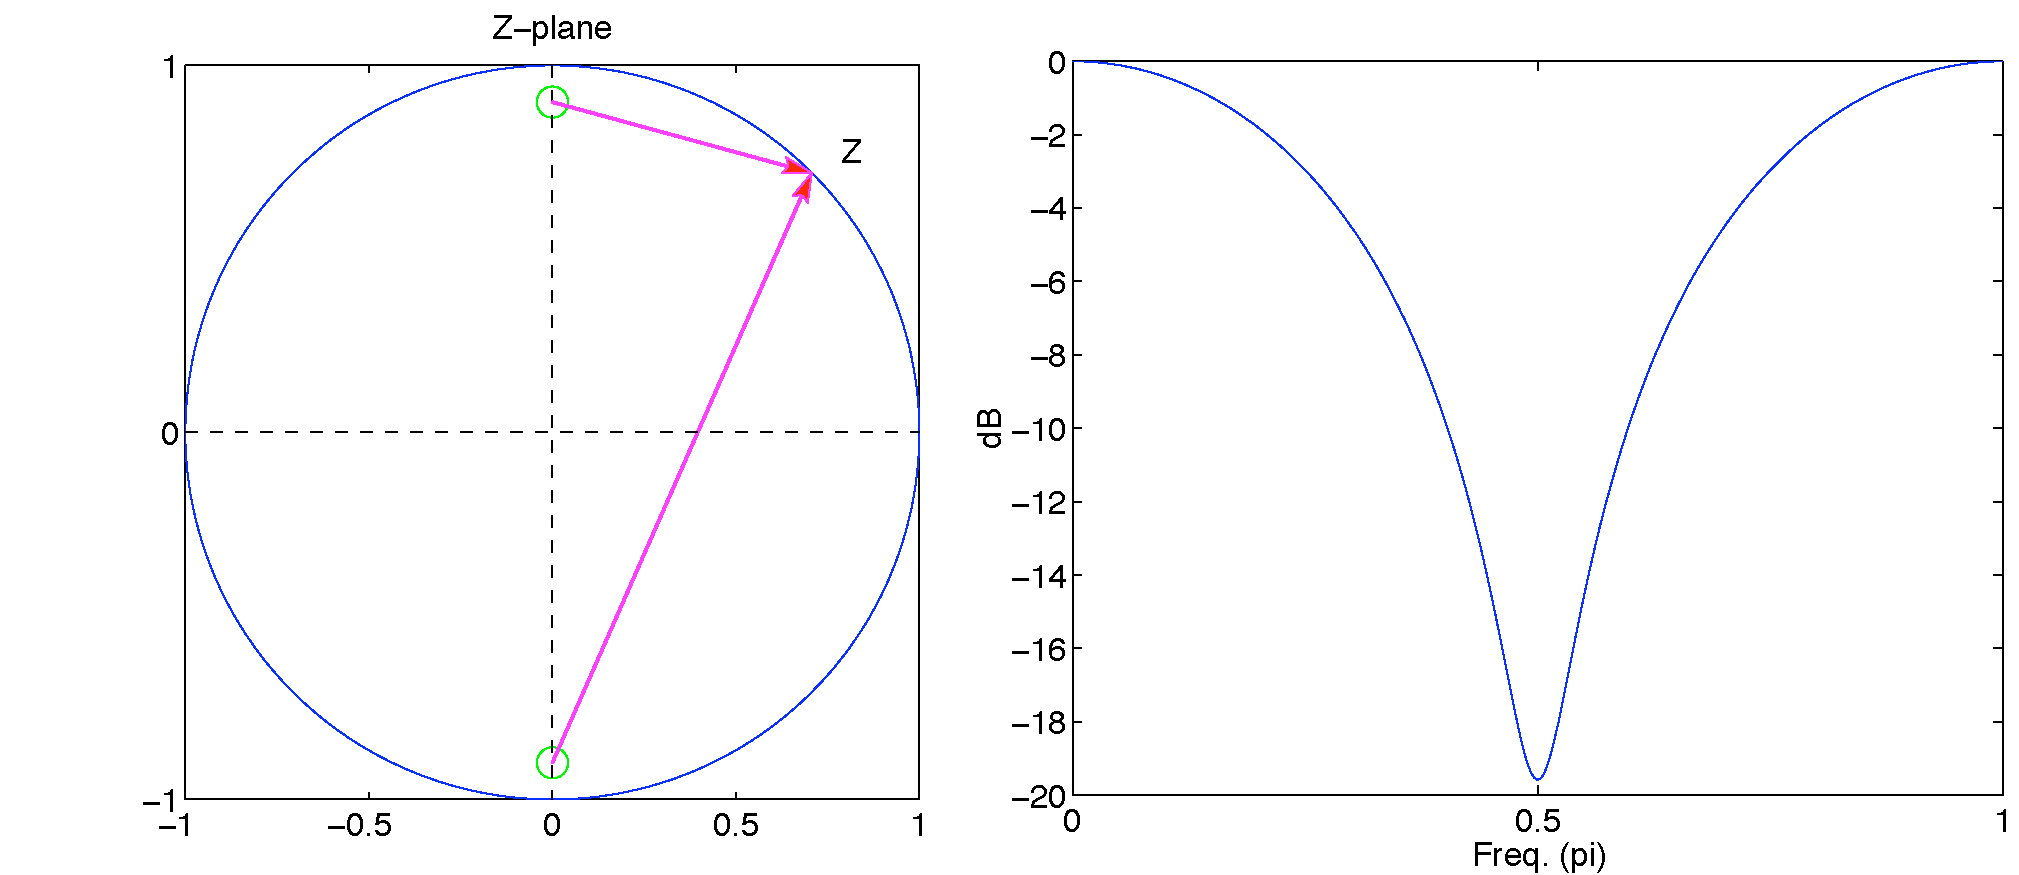
\includegraphics[width=6in]{ch-fir/ffexp_2tdelay_czh90_r0-9}}
\caption[Two zero filter $r=0.9$, $\hat{\omega}_0=\pm\pi/2$.]{Two zero feedforward filter with $r=0.9$, $\hat{\omega}_0=\pm\pi/2$ and magnitude of frequency response.
\label{fig:ff-exp2zs90}}
\end{figure}

\begin{figure}[t]
\centerline{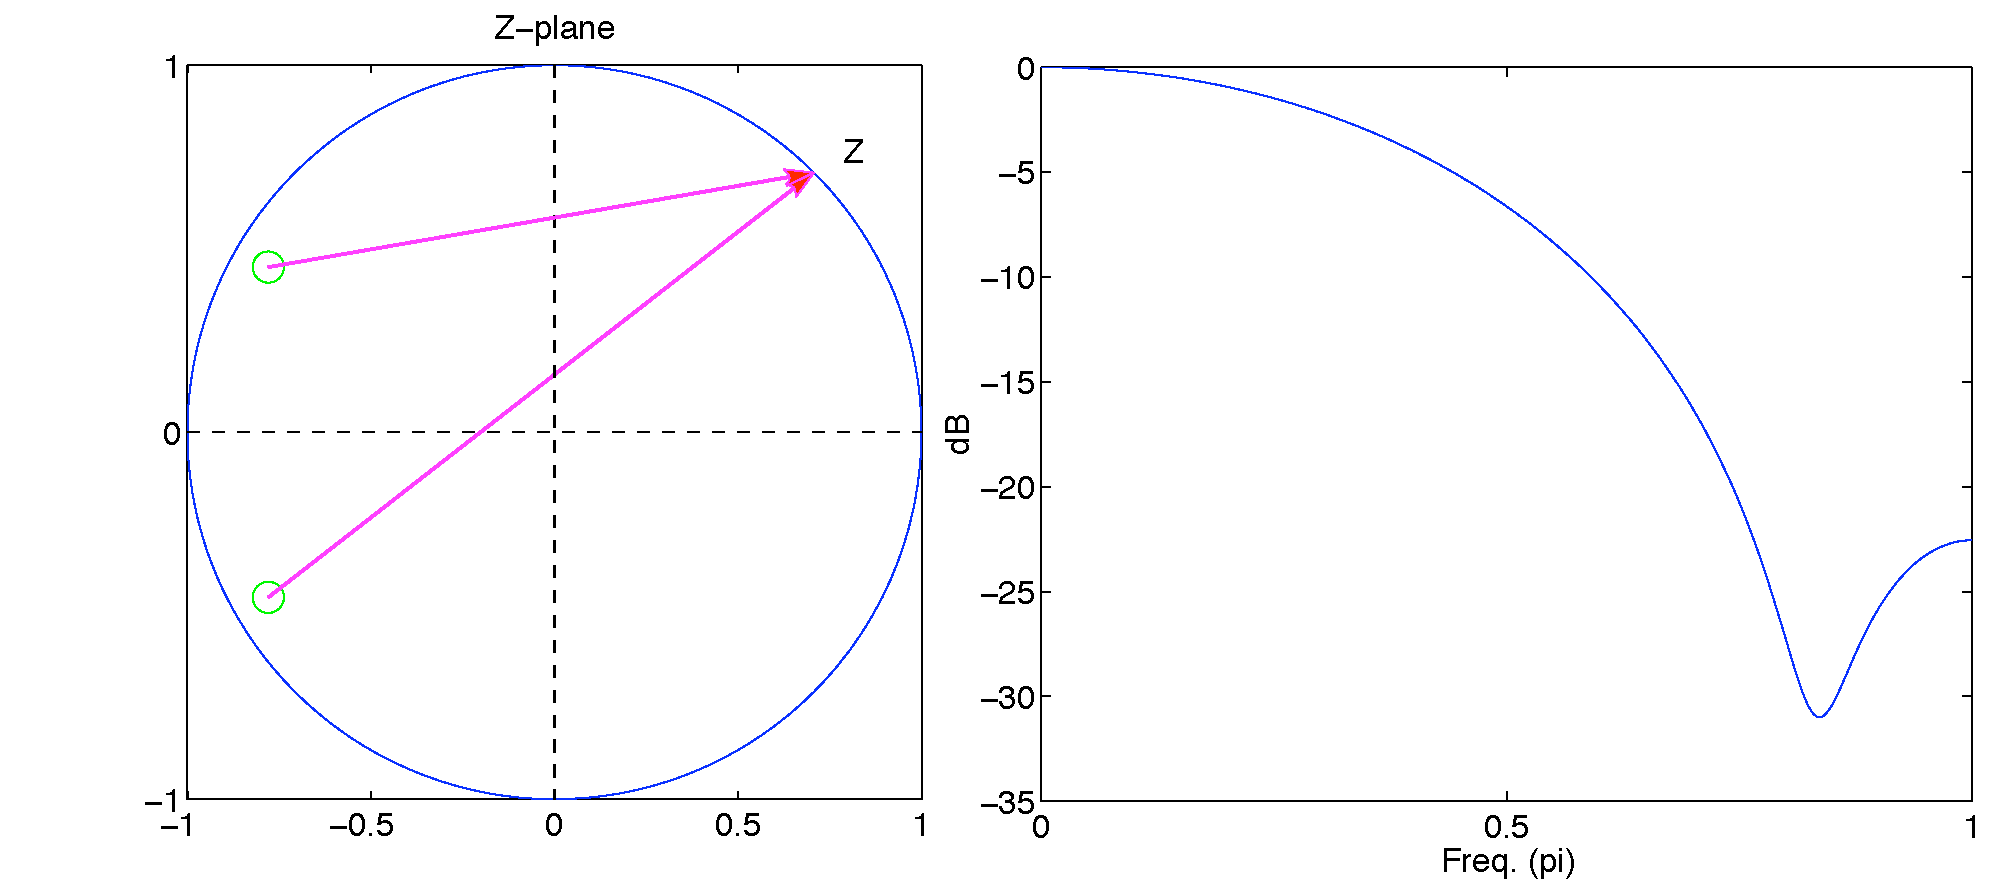
\includegraphics[width=6in]{ch-fir/ffexp_2tdelay_czh150_r0-9}}
\caption[Two zero filter $r=0.9$, $\hat{\omega}_0=\pm5\pi/6$.]{Two zero feedforward filter. $r=0.9$, $\hat{\omega}_0=\pm5\pi/6$ and magnitude of frequency response.
\label{fig:ff-exp2zs150}}
\end{figure}

%\begin{figure}
%\centerline{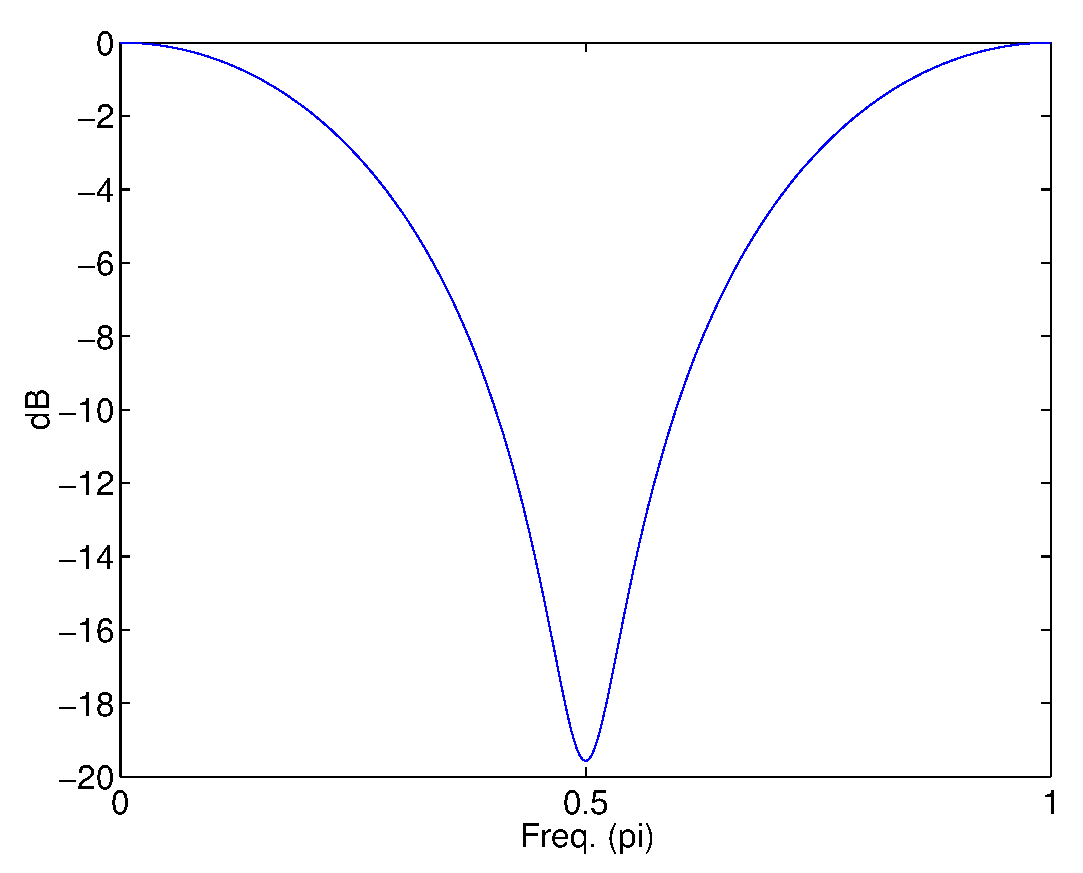
\includegraphics[height=3.5in]{ch-fir/ffexp_2tdelay_h90_r0-9}}
%\caption{Magnitude of frequency response for the filter in
%figure~\protect\ref{fig:ff-exp2zs90}.
%\label{fig:ff-exp2zh90}}
%\end{figure}
%
%\begin{figure}
%\centerline{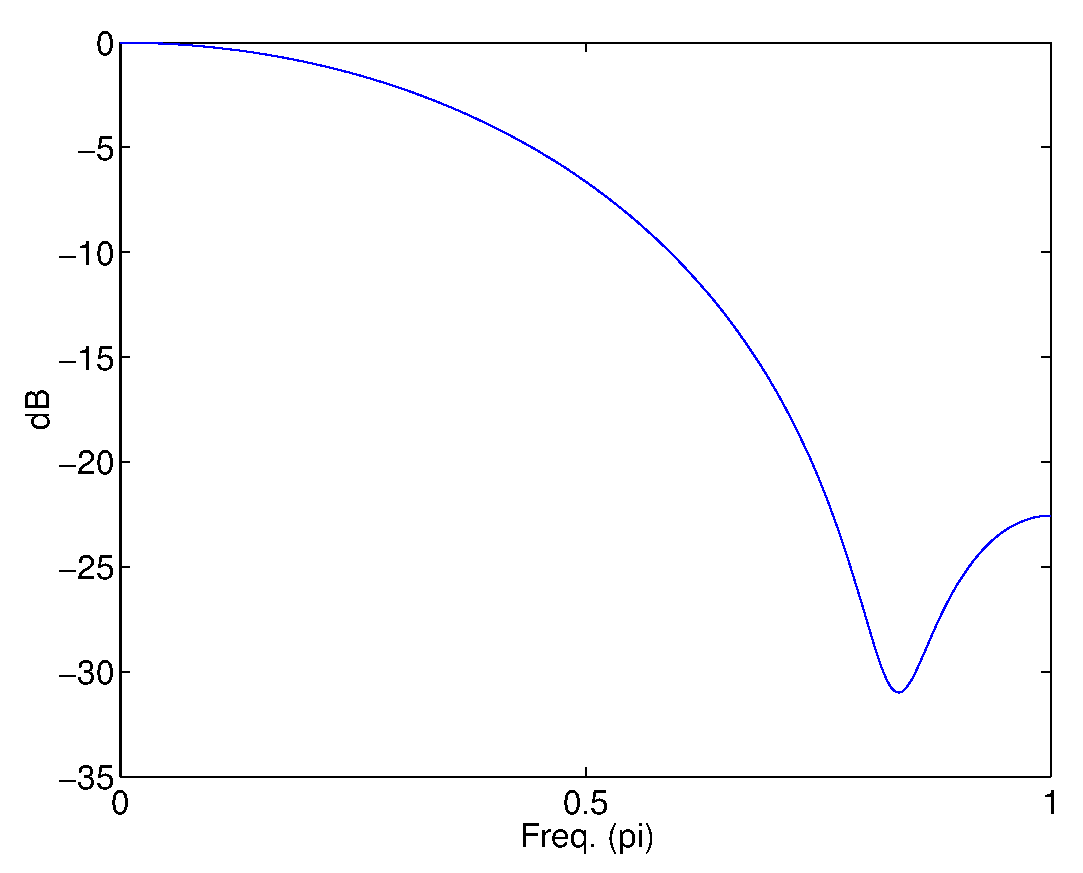
\includegraphics[height=3.5in]{ch-fir/ffexp_2tdelay_h150_r0-9}}
%\caption{Magnitude of frequency response for the filter in
%figure~\protect\ref{fig:ff-exp2zs150}.
%\label{fig:ff-exp2zh150}}
%\end{figure}

We can write the zeros in polar form, for convenience of
visualization, as
\begin{equation}
z_{i}=r_i e^{j \hat{\omega}_{0_i}}, \quad i=1,2
\end{equation}
where $r_i>0$ are the radii where the zeros are located, and
$\hat{\omega}_{0_i}$ their angles.  Depending on the angles
$\hat{\omega}_{0_i}$, the zeros can be either real or complex. For
example, when $\hat{\omega}_{0_i}=0$, the zero lies on the z-plane's
real axis, and when $\hat{\omega}_{0_i}=\pi/2$, it is on the imaginary
axis. Actually, when a filter's coefficients are real, if one of the
zeros is a complex number, the other one will be its conjugate mate
(if one of them is real, the other will be real, too).  So, in the
case where one zero is imaginary at $\hat{\omega}_{0_i}=\pi/2$, the
other zero's angle would be $\hat{\omega}_0=-\pi/2$. So, for this
filter and real coefficients, the pair of complex zeros can be written
as
\begin{equation}
z_{1,2}=r e^{\pm j \hat{\omega}_0}
\label{eq:ff-zero}
\end{equation}

Figures~\ref{fig:ff-exp2zs90} and~\ref{fig:ff-exp2zs150} show two
different sets of zero locations. The magnitude responses for
those two sets of zeros are also presented.

\subsection{Phase Response}

\index{filter!phase response|(emph}
So far we have been talking about the magnitude response of
$\mathcal{H}(\hat{\omega})$.  In the last topic of this chapter, let's
talk about is its phase response. We already know that
$\mathcal{H}(\hat{\omega})$ can be expressed in polar form, with its
magnitude and angle
\begin{equation}
\mathcal{H}(\hat{\omega})=|\mathcal{H}(\hat{\omega})|e^{j \theta(\hat{\omega})}
\end{equation}
$|\mathcal{H}(\hat{\omega})|$ is the magnitude response and
$\theta(\hat{\omega})$ is the phase response. The phase response can
be computed as
\begin{equation}
\theta(\hat{\omega}) = \angle\mathcal{H}(\hat{\omega})
 = \arctan\left(\frac{\Imag[\mathcal{H}(\hat{\omega})]}{\Real[\mathcal{H}(\hat{\omega})]}\right)
\label{eq:compute-phase-resp}
\end{equation}

When the input signal is a phasor, $x[n]=e^{jn\hat{\omega}}$, the
filter's output is
\begin{equation}
y[n] = \underbrace{|\mathcal{H}(\hat{\omega})|e^{j
    \theta(\hat{\omega})}}_{\mathcal{H}(\hat{\omega})} e^{jn\hat{\omega}}
= \underbrace{|\mathcal{H}(\hat{\omega})|}_{\text{change in magnitude}}
  \underbrace{e^{j(n\hat{\omega} +
      \theta(\hat{\omega}))}}_{\text{phase shift}}
\end{equation}
So, what a filter does to a phasor (one frequency of the input) is to
change the input's magnitude at that frequency by multiplying by
$|\mathcal{H}(\hat{\omega})|$ and shift its phase (which is the same
thing as delaying it) by the phase response $\theta(\hat{\omega})$.
\index{filter!phase response|)}

\paragraph*{Example 4:}

Let's examine the previous example (from the discussion of the z-plane):
\begin{equation*}
y[n] = x[n] + b_1x[n-1] + b_2x[n-2]
\end{equation*}
Its transfer function is
\begin{equation*}
H(z)=1 + b_1z^{-1} + b_2z^{-2} 
\end{equation*}
with the values $b_1=0$ and $b_2=1$. The frequency response can be separated into the magnitude and phase response according to,
\begin{align}
\mathcal{H}(\hat{\omega}) &= 1 + b_1e^{-j\hat{\omega}} + b_2e^{-2j\hat{\omega}}
\label{eq:ff-2zthosimple} \\
&= 1 + e^{-2j\hat{\omega}}  && (\text{substitute for $b_1, b_2$}) \notag\\
&= e^{-j\hat{\omega}} (e^{j\hat{\omega}}  + e^{-j\hat{\omega}})  &&
 (\text{factor out $e^{-j\hat{\omega}} $}) \notag \\
&=\underbrace{e^{-j\hat{\omega}}}_{\stackrel{\text{phase}}{_\text{response}}} 
\underbrace{2\cos(\hat{\omega})}_{\stackrel{\text{magnitude}}{_\text{response}}}  &&
 (\text{use Euler's formula}) \label{eq:ex4final}
\end{align}
The magnitude of equation~(\ref{eq:ex4final}) is:
\begin{equation}
|\mathcal{H}(\hat{\omega})|=2|\cos(\hat{\omega})|
\label{eq:ff-z0ssimp}
\end{equation}
and the phase is 
\begin{align}
\theta(\hat{\omega})
              &= \left\{\begin{array}{rl}
                         -\hat{\omega} & 0 \leq \hat{\omega} < \pi/2\\
                         \pi-\hat{\omega} & \pi/2 < \hat{\omega} \leq \pi
                        \end{array}\right.
                        \label{eq:ff-z0phasesimp}
\end{align}
Notice there is a jump of $\pi=180^\circ$ when the $\cos\hat{\omega}$ goes from positive to negative at $\hat{\omega}=\pi/2$. 

In other words \emph{both} the magnitude and phase responses are
functions of $\hat{\omega}$ --- they change the input in a
frequency-dependent way. According to equation~(\ref{eq:ff-z0ssimp}), the
two zeros of the transfer function are at:
\begin{equation*}
\hat{\omega}= \pm\frac{\pi}{2}
\end{equation*}
which, in the z-plane, are a pair of complex zeros on the imaginary axis. Using polar
coordinates they are
\begin{equation}
z_{1,2} = e^{\pm j\pi/2}
\end{equation}
with $r=1$. 

We can illustrate the effect of this filter in a simple manner by
examining the response when the input is a phasor (a single frequency,
$x[n]=e^{jn\hat{\omega}}$):
\begin{equation}
  y[n]= \mathcal{H}(\hat{\omega})x[n] 
      = 2\cos\hat{\omega} e^{j(n-1)\hat{\omega}} \label{eq:ff-2zt}
\end{equation}
We can see that the effect of the filter on the input signal is to
delay it by one sampling interval (from the $(n-1)$ term in the
exponential) and to multiply it by $2\cos\hat{\omega}$. Notice that
the delay is independent of its frequency. When all the frequency
components of a signal are delayed by an equal amount, say the filter
has \emph{no phase distortion} or \emph{linear phase}. The magnitude response and phase response are
shown in figure~\ref{fig:ff-exp2zh90-r1}.

\begin{figure}
\centerline{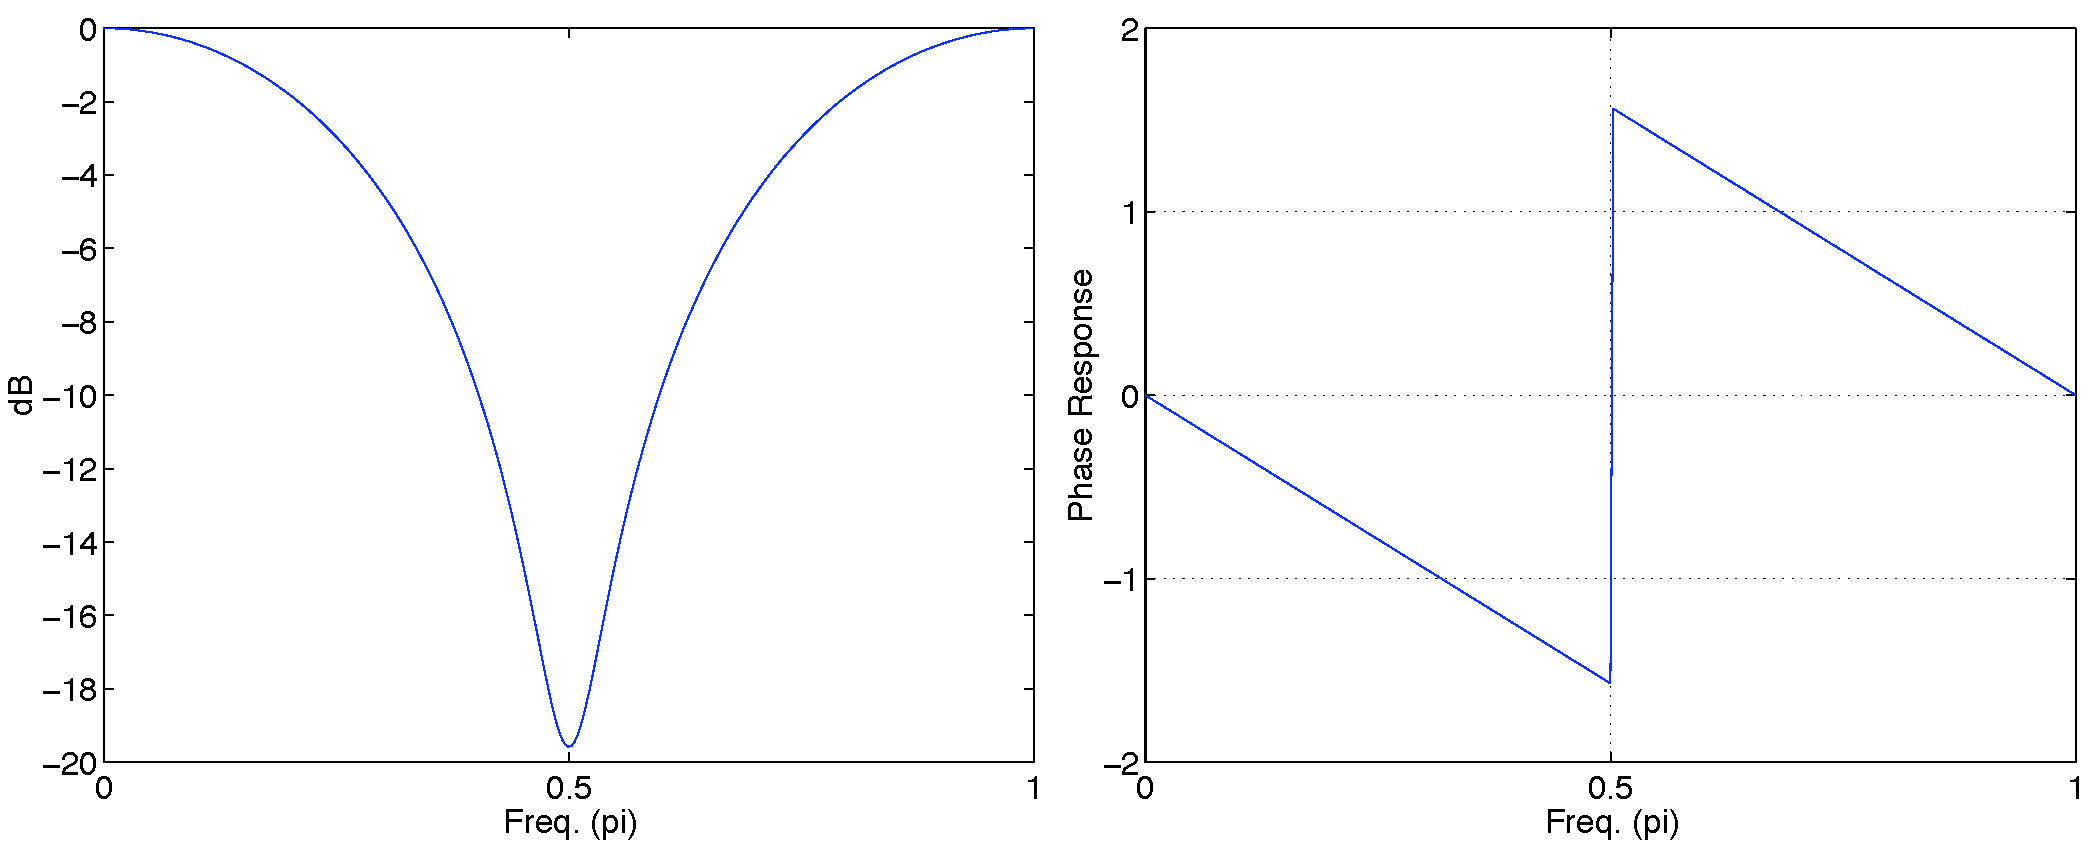
\includegraphics[width=6in]{ch-fir/ffexp_2tdelay_h90}}
\caption[Frequency response of two time delay feedforward
filter]{Magnitude and phase response of two time delay feedforward filter, with
$b_1=0, b_2=1$ in~(\protect\ref{eq:ff-2zt}).  Its zeros are at $e^{\pm
j\pi/2}$.
\label{fig:ff-exp2zh90-r1}}
\end{figure}

\paragraph*{Example 4: generic method [optional]}
There is also a more generic method to get the filter's phase response that will work for any value of $b_1$ and $b_2$, for which we need to access the frequency
response's real and imaginary parts. The frequency response
is
\begin{align}
\mathcal{H}(\hat{\omega}) &= 1 + b_1e^{-j\hat{\omega}} + b_2e^{-2j\hat{\omega}}
\label{eq:ff-2ztho} \\
     &= 1 + b_1(\cos\hat{\omega} - j\sin\hat{\omega})
        + b_2(\cos 2\hat{\omega} - j\sin 2\hat{\omega})
\notag \\
     &= \underbrace{(1 +b_1\cos\hat{\omega}+b_2\cos
       2\hat{\omega})}_{\Real[\mathcal{H}(\hat{\omega})]}
        \underbrace{-j(b_1\sin\hat{\omega}+b_2\sin
          2\hat{\omega})}_{j\Imag[\mathcal{H}(\hat{\omega})]}
\notag
\end{align}
where we have used Euler's formula to rewrite it so that we can
separate its real and imaginary components. We can obtain the
magnitude response from the square root of the sum of the square of
these components and the phase response using
equation~(\ref{eq:compute-phase-resp}).

When the magnitude response of a filter is plotted, the $y$ axis scale
is usually expressed in decibels (dB), a logarithmic scale. We can
take advantage of this to slightly simplify its
computation.  To do this, we note that the \emph{square} of the
magnitude response is the sum of the squares of the real and imaginary
components:
\begin{equation}
|\mathcal{H}(\hat{\omega})|^2=[1 +b_1\cos\hat{\omega}+b_2\cos 2\hat{\omega}]^2 +
              [b_1\sin\hat{\omega}+b_2\sin 2\hat{\omega}]^2
\label{eq:ff-exph1}
\end{equation}

\index{decibel}
A quantity is converted to dB by taking twenty times the logarithm
(base ten).  $|\mathcal{H}(\hat{\omega})|$ can be converted to dB as
\begin{align*}
|\mathcal{H}(\hat{\omega})|_{\mathit{dB}} &= 20\log_{10}|\mathcal{H}(\hat{\omega})|=10\log_{10}|\mathcal{H}(\hat{\omega})|^2
\\
           &= 10\log_{10}\left\{[1 +b_1\cos\hat{\omega}+b_2\cos 2\hat{\omega}]^2 +
               [b_1\sin\hat{\omega}+b_2\sin 2\hat{\omega}]^2\right\}
\end{align*}
Which is a trivial matter to compute for any value of $\hat{\omega}$ (on a
computer) for plotting purposes.  The phase response is
\begin{equation}
\theta(\hat{\omega})=\arctan\left[\frac{-(b_1\sin\hat{\omega}+b_2\sin 2\hat{\omega})}
                            {1 +b_1\cos\hat{\omega}+b_2\cos 2\hat{\omega}}\right]
\label{eq:ff-expph1}
\end{equation}

Consider the special case used in the previous example: $b_1=0$ and $b_2=1$ (a filter with a two-step
delay). Substituting these values into equations~(\ref{eq:ff-exph1})
and~(\ref{eq:ff-expph1}), the squared magnitude becomes
\begin{align*}
|\mathcal{H}(\hat{\omega})|^2 &= (1+\cos 2\hat{\omega})^2 + \sin^2 2\hat{\omega} \\
             &= 1+2\cos 2\hat{\omega}+\cos^2 2\hat{\omega}+\sin^2 2\hat{\omega} \\
             &= 1+2\cos 2\hat{\omega} + 1 \\
             &= 2(1+\cos 2\hat{\omega}) \\
             &= 2(1+2\cos^2 \hat{\omega}-1) \\
             &= 4\cos^2 \hat{\omega}
\end{align*}
Where the next to last step made use of the double-angle identity,
$\cos 2\theta = 2\cos^2 \theta - 1$.  The square root of this is
\begin{equation*}
|\mathcal{H}(\hat{\omega})|=2|\cos \hat{\omega}|
\end{equation*}
Which is exactly what we calculated in equation (\ref{eq:ff-z0ssimp})!

With the substitution, the phase response becomes
\begin{equation}
\theta(\hat{\omega})=\arctan\left(\frac{-\sin 2\hat{\omega}}{1+\cos 2\hat{\omega}}\right)
\label{eq:ff-expph2}
\end{equation}
If we remember the double-angle formulae,
\index{trigonometry!double-angle formulae}
\begin{align*}
\sin 2\hat{\omega} &= \frac{2\tan\hat{\omega}}{1+\tan^2\hat{\omega}} \\
\cos 2\hat{\omega} &= \frac{1-\tan^2\hat{\omega}}{1+\tan^2\hat{\omega}}
\end{align*}
and substitute them into equation~(\ref{eq:ff-expph2}), we get
\begin{align*}
\theta(\hat{\omega})&= \arctan\left(\frac{-2\tan\hat{\omega}}{2}\right) \\
              &= \arctan(-\tan\hat{\omega})\\
              &= \left\{\begin{array}{rl}
                         -\hat{\omega} & 0 \leq \hat{\omega} < \pi/2 \\
                         \pi-\hat{\omega} & \pi/2 < \hat{\omega} \leq \pi
                        \end{array}\right.
\end{align*}
Which is what we calculated in equation (\ref{eq:ff-z0phasesimp}). 

The final result for the transfer function, written in
polar form, is:
\begin{equation}
\mathcal{H}(\hat{\omega}) = |\mathcal{H}(\hat{\omega})|e^{j\theta(\hat{\omega})} = 
e^{-j\hat{\omega}}2\cos\hat{\omega} 
\label{eq:ff-2zth}
\end{equation}


\problemset{
\subsubsection{Self-Test Exercises}

See~\ref{sc:ch3ex} \#\ref{it:ch3ex6}--\ref{it:ch3ex7} for answers.

\begin{enumerate}
\item Prove $|z^2|=1$ in
  equation~(\ref{eq:twostep-ex}).
\item Starting with the factored magnitude response in
  equation~(\ref{eq:twostep-factored}), derive expressions for $b_1$
  and $b_2$ in terms of $z_1$ and $z_2$.
\end{enumerate}}

\subsection{Implementing Digital Filters}

\index{digital filtering!pseudocode|(}
Implementing feedforward digital filters is really quite
straightforward. Let's first look at how we would implement the two
time delay feedforward filter $y[n]=x[n]+b_1x[n-1]+b_2x[n-2]$, when
$b_1=0, b_2=1$, using pseudocode.  I'll present segments of a script
to do the computation and plot some results with my comments on it
interspersed.

\begin{algorithm}
\caption{Generate two sinusoids.\label{alg:gensine}}
\begin{algorithmic}
\STATE $F_s=100$, $N=100$, $T_s=1/F_s$
\STATE $f_1=5$ and $f_2=25$
\FOR{$n=0, 1, 2, \ldots N-1$}
   \STATE $x[n] = \sin(2\pi f_1 n T_s)+\sin(2\pi f_2 n T_s)$
\ENDFOR
\end{algorithmic}
\end{algorithm}

%\begin{small}
%\begin{verbatim}
%% exp_ff_filter.m				
%% feedforward filter : y_t = x_t + b1x_t + b2x_t
%% when a1=0, a2=1;
%
%clf;
%clear
%
%% --- Generate an input signal --- 
%Fs=100;                 % Sampling frequency Fs, samples/second
%N=100;                  % make N samples
%Ts = 1/Fs;              % time interval, seconds/sample
%t = (1:N)*Ts;           % discrete time axis (sample times, in seconds)
%f1 = 5;                 % input signal's frequency
%f2 = 25;
%b1 = 0;                 % filter coefficients
%b2 = 1;
%x=sin(2*pi*t*f1)+sin(2*pi*t*f2);      % input signal 
%\end{verbatim}
%\end{small}

In algorithm~\ref{alg:gensine}, we've generated a discrete signal $x$ containing sine wave values at all the time points at which
the sampling should occur (100 samples at 100Hz = 1 second). The
signal has two frequency components: one at 5Hz and one at 25Hz (both
well below the Nyquist frequency).

\begin{algorithm}
\caption{Filtering.\label{alg:filtering}}
\begin{algorithmic}
\STATE $b_1=0$ and $b_2=1$
\STATE $y[0]=0$ and $y[1]=0$
\FOR{$n=2, 3, 4  \ldots N-1$}
   \STATE $y[n] = x[n]+b_1x[n-1]+b_2x[n-2]$
\ENDFOR
\end{algorithmic}
\end{algorithm}
%\begin{small}
%\begin{verbatim}
%% --- Filtering ---
%y = zeros(size(x));
%y(3:N) = x(3:N) + b1*x(2:N-1) + b2*x(1:N-2);
%y = real(y);
%\end{verbatim}
%\end{small}

In algorithm~\ref{alg:filtering}, we have the luxury of being able to
hold the entire input and output signal in arrays. Because there is a two time step delay, we
can't compute a value for $y[0]$ or  $y[1]$, so those are set to zero. 

%\begin{algorithm}
%\caption{Calculate spectra.\label{alg:spectra}}
%\begin{algorithmic}
%\STATE $X$=\verb|fft|($x$), take 512 point fast Fourier transform of $x$
%\STATE $Y$=\verb|fft|($y$), take 512 point fast Fourier transform of $y$
%\FOR{$k=0, 1, 2,  \dots 256$}
%   \STATE Plot abs($X[k]$) and abs($Y[k]$) at frequency $k\times F_s/512$
%\ENDFOR
%\end{algorithmic}
%\end{algorithm}

%\begin{small}c  x
%\begin{verbatim}
%% --- plot magnitude of the input and output signals' spectra ---
%spx=fft(x,512);         % original signal's fft
%spy=fft(y,512);
%fstep=(Fs/2)/256;       % frequency step
%f=(0:255)*fstep;        % frequency axis
%plot(f,abs(spx(1:256)'), 'g', f,abs(spy(1:256)'), 'm');
%                        %plot spx and spy in the same plot
%xlabel('Freq. (Hz)', 'Fontsize', 16);
%ylabel('Freq. Components', 'Fontsize', 16);
%set(gca, 'Fontsize', 16);
%input('Press key to continue')
%\end{verbatim}
%\end{small}

%TODO replace with intuition
After we filter the sum of sinusoids, we want to see what happened to the signal's frequency components. We will use the fast Fourier Transform to analyze the components. We'll talk about
the Fourier transform and FFT in section~\ref{sc:fourier-xform}.
Figure~\ref{fig:ff-expsin2_sp} shows the magnitude of each frequency in the generated and filtered sine waves. From the plot we can see that the high frequency wave is completely filtered out. And finally, we'll plot the input and output. They're shown in
figure~\ref{fig:ff-expsin2_sp} (right).

%\begin{small}
%\begin{verbatim}
%% --- Plot orignal and filtered signal ---
%plot(t, x, 'b', t, y, 'r' );
%xlabel('Time (sec)', 'FontSize', 16);
%ylabel('Time waveform', 'FontSize', 16);
%set(gca, 'FontSize', 16);
%\end{verbatim}
%\end{small}
%\index{MATLAB code!digital filtering|)}

How would one implement this in a language like C, C++, Java, etc?
Let's not worry about the plotting issue: that would certainly have to
be dealt with, but it would involve either getting a graphics library,
writing one's own, or using an external plotting package (ideally, one
targeted at scientific and engineering applications, rather than one
written for business).  For example, a fine alternative would be to 
vectorize all the array operations and use MATLAB.  We will
discuss the \verb|fft()| function in section~\ref{sc:fft}. The
only remaining issue is that of keeping the entire input and output
signal in memory.
\begin{figure}
\centerline{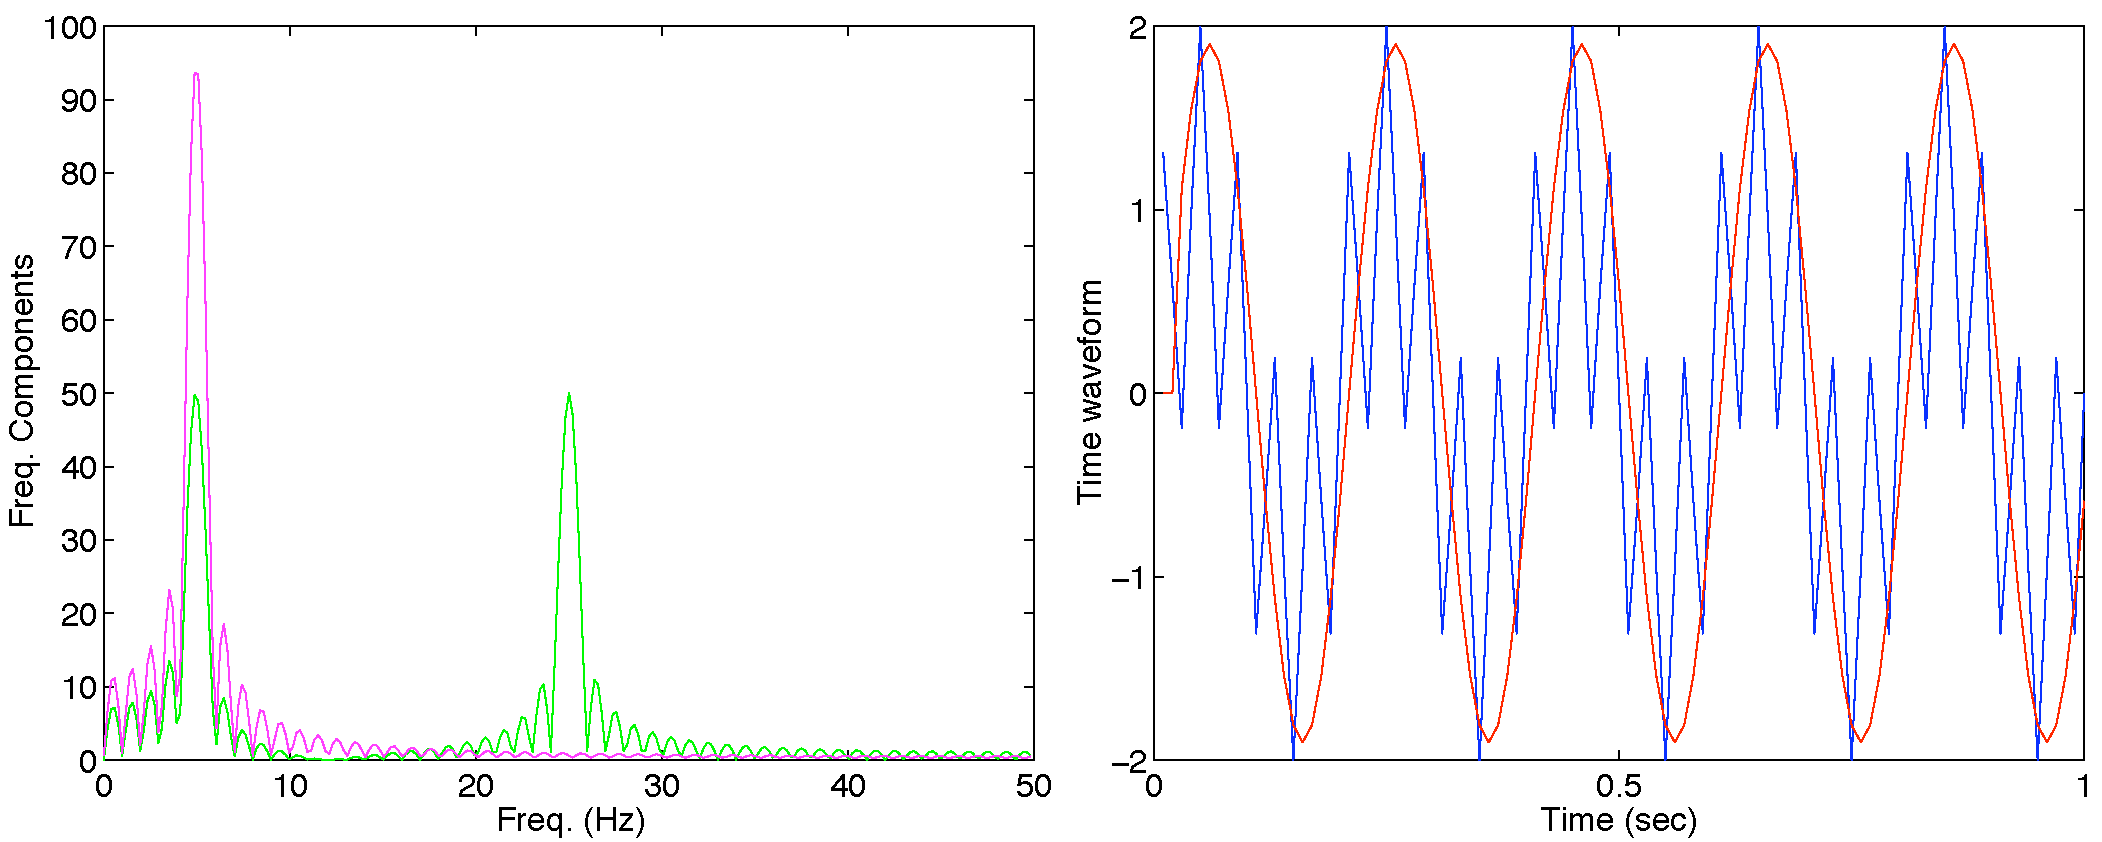
\includegraphics[width=6in]{ch-fir/sine2_ff2td_sp_wv}}
\caption[Two sinusoid spectrum]{The spectrum of a two frequency component sine wave and its filtered version,
using the feedforward filter $y[n]=x[n]+x[n-2]$, $f_1=5Hz$ and
$f_2=25Hz$. Zeros are at $z_0=0.99e^{\pm j\pi/2}$. The time waveforms are also shown.
\label{fig:ff-expsin2_sp}}
\end{figure}

%\begin{figure}
%\centerline{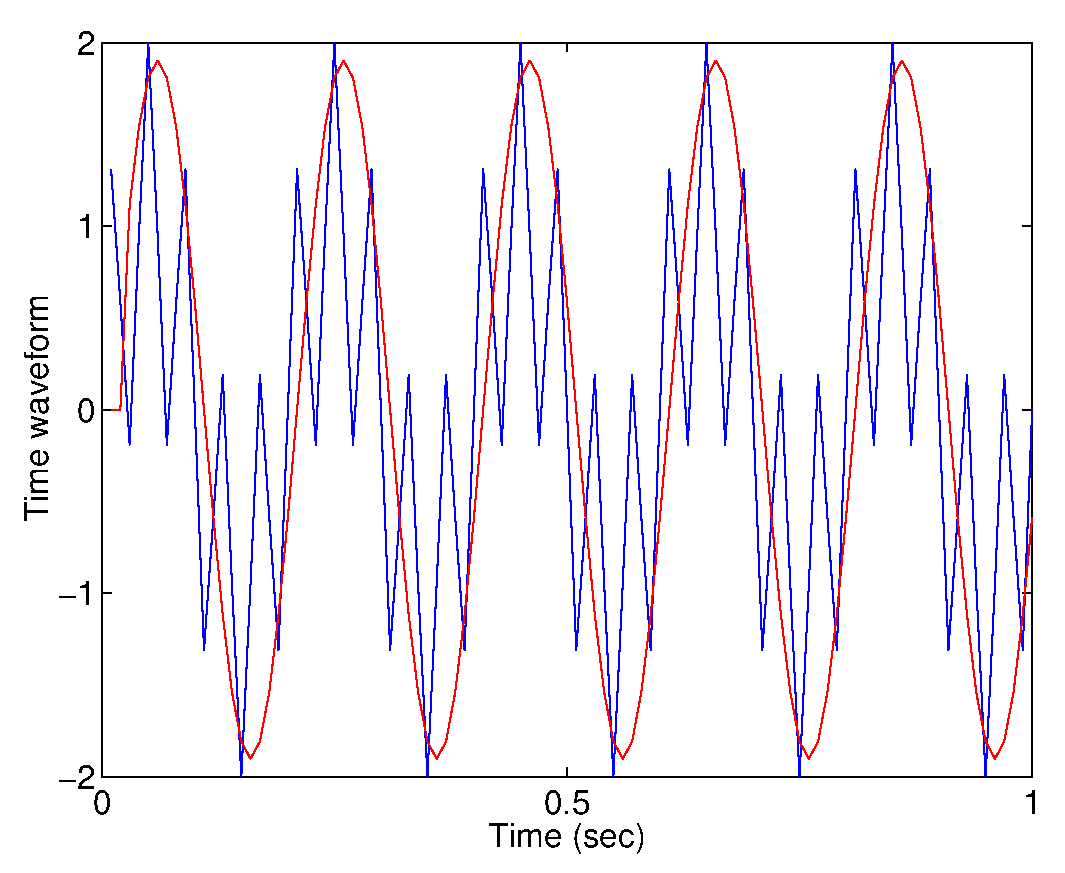
\includegraphics[width=4in]{ch-fir/sine2_ff2td}}
%\caption[Two frequency component sine wave and its filtered
%version]{Two frequency component sine wave and its filtered version,
%using the feedforward filter $y[n]=x[n]+x[n-2]$, $f_1=5Hz$ and
%$f_2=25Hz$. Zeros are at $z_0=0.99e^{\pm j\pi/2}$.
%\label{fig:ff-expsin2}}
%\end{figure}
In general, it is not possible to keep the entire input and output
signal in memory. In fact, many (if not most) digital signal
processing applications involve real-time processing, so the computer
system really needs to be viewed as just a stage in a processing
pipeline, with the input flowing in and the output flowing out (just
like the block diagrams used to illustrate filters).  We can therefore
only devote a relatively small amount of memory to hold the part of
the input and output needed for the current computation. If $n$
delayed samples of the input are needed to compute each output value,
we will need storage for $n+1$ input samples (the current one plus the
delayed samples). For a feedforward filter, there is no need to save
output values; they can be sent out as soon as they are computed.

What abstract data type (ADT) should hold the delayed inputs (answer
in~\ref{sc:ch3ex} \#\ref{it:ch3ex8})?  As each input sample comes in,
it displaces the oldest input sample from our buffer of $n+1$
values. For computer scientists, this is clearly a first-in-first-out (FIFO) ADT --- a \emph{queue}. A queue is very efficiently and simply implemented in an
array, especially when the queue size is fixed. Furthermore, you
can treat the array as though it were circular
using indexing modulo the queue size.

\section{Problems}

\begin{enumerate}
\item In Example~4, we used a large number of trigonometric identities
  to go from the filter's frequency response in~(\ref{eq:ff-2ztho}) to
  the results in~(\ref{eq:ff-2zth}) and~(\ref{eq:ff-2zt}) for the
  special case of $b_1=0$ and $b_2=1$. There is an easier way. First,
  substitute the values of $b_{1,2}$ into~(\ref{eq:ff-2ztho}), and then
  use the fact that we can always factor a real number into a product of
  complex conjugate numbers, i.e., $1 = e^{j\hat{\omega}}
  e^{-j\hat{\omega}}$. A little bit of algebra and Euler's formula
  should allow you to derive the results (\ref{eq:ff-2zth}) and
  (\ref{eq:ff-2zt}) of Example~4 much easier.
\item For the filter whose magnitude response is described
  in~(\ref{eq:twostep-factored}), plot the location of a pair of complex
  conjugate zeros at $r=0.8$ and $\hat{\omega}_0=\pm\pi/4$. Using MATLAB,
  compute and plot the filter's magnitude response. Submit your code
  with your figures.
\item In the self-test exercise on page~\pageref{sc:ste-oper}, two
  filters with transfer functions $H_1(z) = b_0 + b_1z^{-1}$ and
  $H_2(z) = b'_0 + b'_1z^{-1}$ were connected in series, and it was
  shown that they could be connected in either order to produce the same
  composite effect (the same overall transfer function). Redo this
  exercise using the defining equations for the two filters, i.e.,
  $y_1[n] = F_1(x[n])$ for the filter with transfer function $H_1(z)$
  and $y_2[n] = F_2(x[n])$ for the filter with transfer function
  $H_2(z)$. In other words, show that $F_2(F_1(x[n])) =
  F_1(F_2(x[n]))$.
\item Use MATLAB to plot the results of filtering the following
  signals with the filter: $y[n] = x[n] + x[n-1]$.  Submit your code
  with your results.
  \begin{enumerate}
  \item $x[n] = n$
  \item $x[n] = \sin(n\pi/100)$
  \item $\displaystyle
    x[n] = \left\{\begin{array}{ll}+1 & \quad n \bmod 5 \;\mathrm{even}\\
        -1 & \quad n \bmod 5 \;\mathrm{odd}\end{array}\right. $
  \end{enumerate}
\item Check the following factorization: $z^2 - z + 1 = (z -
  e^{j\pi/3}) (z - e^{-j\pi/3})$
\end{enumerate}

\section{Further Reading}

\begin{itemize}
\item James H McClellan, Ronald W. Schafer, and Mark A. Yoder, \textit{DSP
  First: A Multimedia Approach}, Prentice Hall, 1998, ch. 5 (\S
5.1--5.3), 6 (\S 6.1, 6.4--6.7).
\end{itemize}

% LocalWords:  MATLAB feedforward phasor response's

